\section{Experiments}
\label{sec:experiments}

\subsection{Experimental Setup}
\label{sec:experimental-setup}

Table~\ref{tab:experimental-matrix} summarizes the seven evaluated models and
prompting conditions. GPT-5.5 and GPT-4o provide proprietary API-served
reference points, while Mistral Large 3, Gemma 4, and Qwen3.5 provide coverage
of three open-weight model families
\citep{openai2026gpt55,openai2024gpt4o,mistral2025mistral3,
gemmateam2026gemma4,qwenteam2026qwen35}.
The Qwen3.5 4B, 9B, and 27B models form the only within-family size series.

\begin{table*}[t]
  \centering
  \small
  \setlength{\tabcolsep}{6pt}
  \begin{tabular}{@{}p{0.26\textwidth}p{0.26\textwidth}ccc@{}}
    \toprule
    & & \multicolumn{2}{c}{Zero-shot} & Few-shot \\
    \cmidrule(lr){3-4}
    Model snapshot & Access / serving & Full & No inst. & Shots \\
    \midrule
    GPT-5.5 (2026-04-23) & Proprietary; gateway & \checkmark & \checkmark & 1, 3 \\
    GPT-4o (2024-11-20) & Proprietary; gateway & \checkmark & \checkmark & --- \\
    Mistral Large 3 (2512) & Open-weight; gateway & \checkmark & \checkmark & --- \\
    Gemma 4 31B IT & Open-weight; local vLLM & \checkmark & \checkmark & --- \\
    Qwen3.5 27B & Open-weight; local vLLM & \checkmark & \checkmark & 1, 3 \\
    Qwen3.5 9B & Open-weight; local vLLM & \checkmark & \checkmark & 1, 3 \\
    Qwen3.5 4B & Open-weight; local vLLM & \checkmark & \checkmark & 1, 3 \\
    \bottomrule
  \end{tabular}
  \caption{Model and condition coverage. All seven snapshots are run
  zero-shot under both the full-instruction and no-instruction variants;
  four are additionally run with fixed one- and three-example prompts
  with full field instructions. In the reported evaluation, all 22 conditions
  are scored on the same 30 evaluation papers, yielding 660 paper-level
  extractions.}
  \label{tab:experimental-matrix}
\end{table*}


We use zero-shot extraction with the designed generic and PaN schemas,
including their detailed field instructions, as the baseline setting. To
assess the contribution of these instructions, we compare against an
ablation in which the per-field \texttt{instructions} arrays are removed.
We further examine whether examples provide additional benefit by
evaluating one-shot and three-shot prompting for GPT-5.5 and the three
Qwen3.5 models, using fixed demonstrations drawn from the calibration set.

All conditions use a common text-to-JSON extraction pipeline. PDFs are
converted to Markdown-like text with \texttt{pymupdf4llm}, and models receive
the extracted document text together with the schemas and a common extraction
template. Detailed pipeline and serving settings are reported in
Appendix~\ref{app:reproducibility}.

\subsection{Annotation Agreement}
\label{sec:annotation-agreement}

We measure agreement between two independent annotations of each of the 30
evaluation papers using the entity-aware protocol from
Section~\ref{sec:evaluation}. For funding, samples, and datasets, correspondence 
is established through reconciled gold identities. Entity F1 is symmetric under 
annotator-role reversal. Table~\ref{tab:iaa-recovery} reports entity-level agreement 
for the six entity collections. Agreement is perfect for authors and affiliations, 
whose identities  have direct textual anchors in the publication, and remains high 
but imperfect for funding. Agreement is lower for facilities, samples, and datasets, 
where  annotators must additionally decide whether different mentions, states, or 
measurements constitute the same entity or distinct entities.

\begin{table}[t]
  \centering
  \small
  \begin{tabular}{@{}lrrr@{}}
    \toprule
    Entity collection & F1 & Matched & Unmatched \\
    \midrule
    Affiliations & 1.000 & 133 & 0 \\
    Authors & 1.000 & 228 & 0 \\
    Funding & 0.889 & 60 & 15 \\
    Facilities & 0.753 & 29 & 19 \\
    Samples & 0.845 & 71 & 26 \\
    Datasets & 0.793 & 69 & 36 \\
    \bottomrule
  \end{tabular}
  \caption{Pairwise agreement on entity recovery outcomes for
  the 30 evaluation papers.}
  \label{tab:iaa-recovery}
\end{table}


Inspection of unmatched entity records helps explain these differences in
agreement. Funding disagreements mainly reflect decisions about 
whether reported sources of support should be included as funding entities. 
For the PaN collections, the dominant differences concern entity granularity:
representing facilities at the host-facility or instrument/beamline level,
distinguishing sample preparations, treatments, or states, and combining
versus splitting related measurements into dataset entities.

Field-level agreement also varies after entity alignment, with particularly
low agreement for free-text sample and dataset descriptions. The complete
profile is reported in Table~\ref{tab:appendix-iaa}.
\begin{table*}[!t]
  \centering
  \small
  \setlength{\tabcolsep}{2.5pt}
  \begin{tabular}{@{}p{0.19\textwidth}rrrrrrr@{}}
    \toprule
    Entity collection & GPT-5.5 & GPT-4o & Mistral & Gemma & Qwen 27B & Qwen 9B & Qwen 4B \\
    \midrule
    Affiliations & 1.000 & 1.000 & 1.000 & 1.000 & 1.000 & 1.000 & 1.000 \\
    Authors & 1.000 & 1.000 & 1.000 & 1.000 & 1.000 & 1.000 & 1.000 \\
    Funding & 0.954 & 0.925 & 0.912 & 0.945 & 0.953 & 0.901 & 0.810 \\
    Facilities & 0.545 & 0.892 & 0.735 & 0.860 & 0.769 & 0.783 & 0.744 \\
    Samples & 0.800 & 0.777 & 0.865 & 0.864 & 0.837 & 0.783 & 0.739 \\
    Datasets & 0.832 & 0.609 & 0.656 & 0.778 & 0.814 & 0.732 & 0.636 \\
    \bottomrule
  \end{tabular}
  \caption{Full-instruction zero-shot entity recovery for the six
  entity collections on the 30 evaluation papers. All values
  are entity F1.}
  \label{tab:zero-shot-recovery}
\end{table*}

\begin{table*}[!t]
  \centering
  \small
  \setlength{\tabcolsep}{4pt}
  \begin{tabular}{@{}p{0.18\textwidth}rrrrrrr@{}}
    \toprule
    Entity collection & GPT-5.5 & GPT-4o & Mistral & Gemma & Qwen 27B & Qwen 9B & Qwen 4B \\
    \midrule
    Affiliations & +0.000 & +0.000 & +0.000 & +0.000 & +0.000 & +0.000 & +0.000 \\
    Authors & +0.000 & +0.000 & +0.000 & +0.000 & +0.000 & +0.000 & +0.000 \\
    Funding & +0.000 & +0.007 & +0.029 & +0.000 & -0.008 & +0.030 & -0.047 \\
    Facilities & -0.152 & -0.020 & -0.049 & -0.055 & +0.052 & +0.116 & +0.154 \\
    Samples & +0.079 & +0.177 & +0.046 & +0.045 & +0.042 & +0.022 & +0.055 \\
    Datasets & +0.074 & +0.209 & +0.164 & +0.124 & +0.259 & +0.212 & +0.082 \\
    \bottomrule
  \end{tabular}
  \caption{Effect of detailed field instructions on entity recovery
  for the six entity collections on the 30 evaluation papers,
  reported as full-instruction minus no-instruction entity F1.
  Positive values favor the full instructions.}
  \label{tab:instruction-effects}
\end{table*}


\subsection{Baseline Results}
\label{sec:baseline-results}

Table~\ref{tab:zero-shot-recovery} reports entity recovery for the seven
full-instruction zero-shot conditions.
Generic metadata are generally extracted consistently across models: author and
affiliation entity recovery is 1.000 for every model, while title, abstract,
author-name, and affiliation-label scores are all close to one
(Table~\ref{tab:appendix-zero-shot}). Funding entity recovery also remains
comparatively strong, although its attribute scores are less uniform. In
contrast, PaN entity recovery is lower and more variable across facilities,
samples, and datasets.

This contrast may partly reflect how the target metadata are represented in
the publication. Titles, abstracts, authors, and affiliations are typically
localized and explicitly delimited, making their extraction closer to
transcription. Funding has distinctive lexical anchors such as grant
identifiers, but still requires decisions about inclusion and funder--grant
attribution. Facilities, samples, and datasets often require entities to
be constructed from distributed mentions, including decisions about facility
hierarchy, prepared sample variants, and distinct measurement campaigns.
Similar identity and granularity decisions also account for many of the
annotation disagreements observed in
Section~\ref{sec:annotation-agreement}. 

Within the PaN layer, relative model performance depends on the entity type.
GPT-4o achieves the highest facility recovery, while the leading
sample results for Mistral and Gemma are close, and GPT-5.5
achieves the highest dataset recovery. Within the Qwen3.5 series, recovery
increases from 4B to 9B to 27B for samples and datasets, whereas facility 
recovery peaks at 9B. This suggests that the association between model size 
and recovery depends on the entity type rather than following a uniform pattern 
across PaN extraction.

Higher entity recovery does not necessarily correspond to higher quality on
aligned entities. Table~\ref{tab:appendix-zero-shot} reports the corresponding
conditional attribute and reference scores. GPT-4o has the highest facility
entity F1 but the lowest aligned facility-name score (0.747). A stronger
contrast appears for datasets: GPT-5.5 has the highest dataset recovery but,
among its aligned datasets, the lowest dataset--facility reference F1 (0.500),
whereas GPT-4o has substantially lower dataset recovery (0.609) but the highest
conditional dataset--facility reference F1 (0.909). These results show
that entity recovery and conditional attribute and reference quality capture
different aspects of model performance, although the conditional scores are 
computed on model-specific aligned subsets and reference scores additionally 
depend on recovery of the referenced entities.

\begin{figure*}[!t]
  \centering
  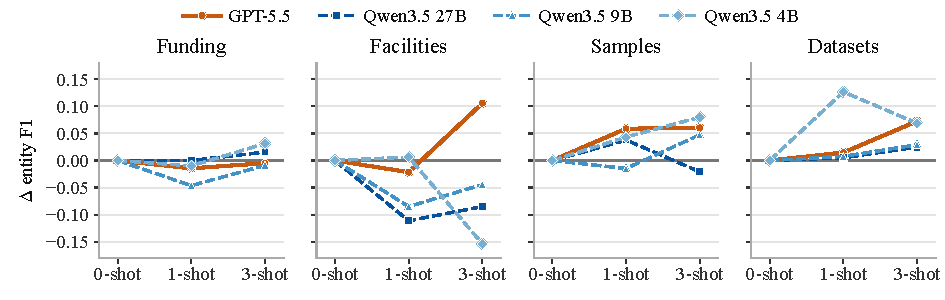
\includegraphics[width=\textwidth]{figures/few_shot.pdf}
  \caption{Effect of fixed demonstrations on entity recovery for the four
  tested models on the 30 evaluation papers, shown as the change in entity F1
  relative to each model's own zero-shot condition (positive values indicate
  higher recovery with demonstrations). Entity F1 for authors and affiliations
  is 1.000 in every condition, so these collections are omitted.}
  \label{fig:few-shot}
\end{figure*}

\subsection{Instruction Ablation}
\label{sec:instruction-ablation}

Table~\ref{tab:instruction-effects} reports the difference in entity F1
between the full-instruction and no-instruction conditions. Detailed instructions
consistently yield higher measured recovery for samples and datasets: dataset
F1 increases by 0.074--0.259 across all seven models, and sample F1 by
0.022--0.177. Author and affiliation recovery is 1.000 with and without
instructions and is therefore unaffected, while funding changes little and in
both directions ($-0.047$ to $+0.030$). Facility recovery shows a different
pattern: instructions reduce F1 for GPT-5.5, GPT-4o, Mistral, and Gemma, but
increase it for all three Qwen3.5 models.

The dataset gains reflect higher recall for six models and
fewer false positives for five. With instructions, six models gain 3--23
dataset true positives; GPT-5.5 retains the same number of true positives and
reduces false positives by 17. False positives are unchanged for Gemma and
increase by one for GPT-4o.

Paired-output inspection suggests that the facility differences partly reflect
how each model's naming and selection behavior interacts with the benchmark's
facility--instrument boundary. The facility instruction requests the specific
facility rather than an umbrella institution, for example PETRA III rather
than DESY, but does not explicitly define the boundary between facilities and
their subordinate instruments or beamlines. For GPT-5.5, Mistral, and Gemma,
instructed outputs often retain an instrument or beamline while omitting the
facility-level name used in the reconciled gold, resulting in fewer recovered
facilities. GPT-4o loses no gold-facility matches; its small F1 decrease comes
from gaining one true positive but three false positives. For all three
Qwen3.5 models, false positives decrease, although their true-positive changes
differ by model. Because the ablation removes the complete instruction bundle
and uses one extraction per paper, these patterns are post hoc explanations
rather than effects isolated to an individual instruction.

\subsection{Few-Shot Demonstrations}
\label{sec:few-shot}

Figure~\ref{fig:few-shot} compares zero-, one-, and three-shot conditions for
GPT-5.5 and the three Qwen3.5 models. Dataset
recovery shows the most consistent three-shot improvement: relative to
zero-shot, entity F1 increases for all four models by 0.025--0.072. Sample
recovery also increases for three of the four models, whereas facility recovery
varies across models and shot counts.

Recovery does not improve monotonically with additional demonstrations.
One-shot and three-shot conditions can move recovery in different directions,
with no consistent ordering across entity types or models. For example,
Qwen3.5 4B dataset F1 rises from 0.636 in zero-shot to 0.763 in one-shot before
decreasing to 0.705 in three-shot, while its sample F1 increases from 0.739 to
0.782 and 0.819. Because only one fixed, ordered set of demonstrations was tested, 
these comparisons characterize the tested prompt configurations and do not isolate 
shot count from exemplar choice.
